\documentclass[12pt, twoside]{article}
\usepackage[letterpaper, margin=1in, headsep=0.5in]{geometry}
\usepackage[english]{babel}
\usepackage[utf8]{inputenc}
\usepackage{amsmath}
\usepackage{amsfonts}
\usepackage{amssymb}
\usepackage{tikz}
%\usetikzlibrary{quotes, angles}

\usepackage{graphicx}
\usepackage{enumitem}
\usepackage{multicol}

\usepackage{fancyhdr}
\pagestyle{fancy}
\fancyhf{}
\renewcommand{\headrulewidth}{0pt} % disable the underline of the header

\fancyhead[RE]{\thepage}
\fancyhead[RO]{\thepage \\ Name: \hspace{3cm}}
\fancyhead[L]{BECA / Dr. Huson / 10th Grade Geometry\\* 19 December 2018}

\begin{document}
\subsubsection*{Homework: Coordinate geometry (due Thursday)}
 \begin{enumerate}

   \item Find the length of $\overline{DE}$, where $D(1,-5)$ and $E(13,0)$.
       \vspace{4cm}

   \item Determine relationship of each equation to the line  $y=\frac{2}{3} x-6$, circling either parallel, perpendicular, or neither.
     \begin{enumerate}
       \item $2x-3y=6$ \hspace{1cm} Parallel \qquad Perpendicular \qquad Neither
       \vspace{1.5cm}
       \item $3x-2y=5$ \hspace{1cm} Parallel \qquad Perpendicular \qquad Neither
       \vspace{2.cm}
     \end{enumerate}

  \item In the diagram below, $\overleftrightarrow{AC}$ has endpoints with coordinates $A(-1,2)$ and $C(8, -4)$.
    \begin{center} %4 quadrant regents grid
      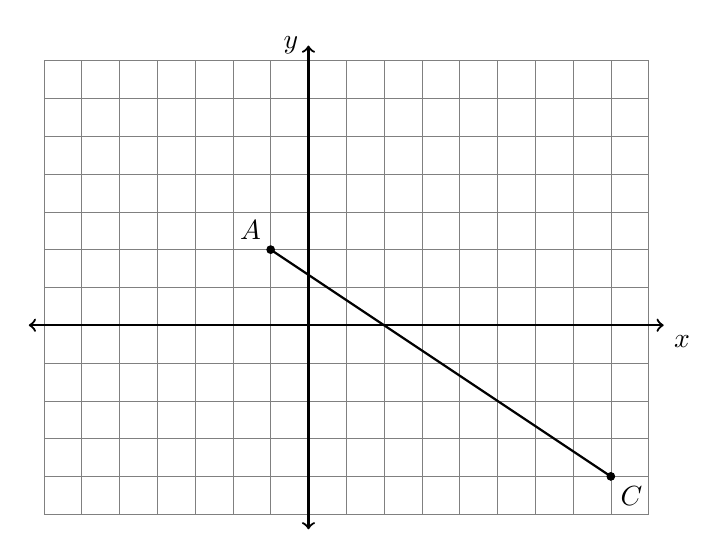
\begin{tikzpicture}[scale=.48]
        \draw [help lines] (-7,-5) grid (9,7);
        \draw [thick, <->] (-7.4,0) -- (9.4,0) node [below right] {$x$};
        \draw [thick, <->] (0,-5.4)--(0,7.4) node [left] {$y$};
        \draw [thick] (-1,2)--(8, -4);
        \draw [fill] (-1,2) circle [radius=0.1] node[above left] {$A$};
        \draw [fill] (8, -4) circle [radius=0.1] node[below right] {$C$};
      \end{tikzpicture}
    \end{center}
    If $B$ is a point on $\overline{AC}$ and $AB {:} BC = 1{:}2$,  what  are  the  coordinates of $B$?

\newpage

\item $A(2,10)$ is one endpoint of $\overline{AB}$. The segment's midpoint is $M(5,7)$. Find the other endpoint, $B$. \vspace{4cm}

\item In the diagram below, $\triangle ABC$ has vertices with coordinates $A(1,3)$, $B(8,4)$ and $C(4, 7)$.
  \begin{center} %4 quadrant regents grid
    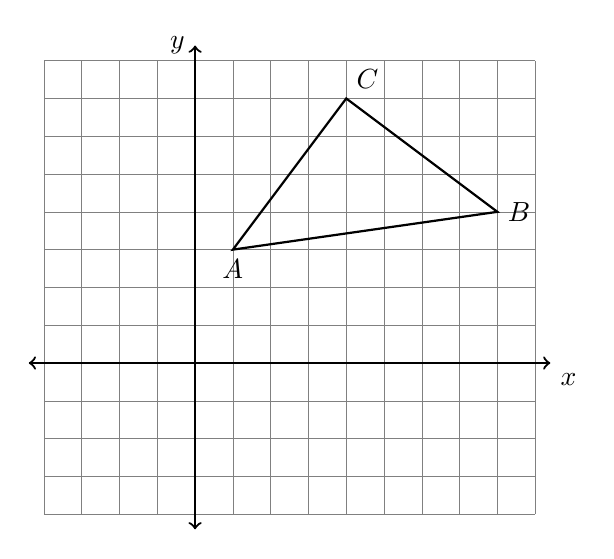
\begin{tikzpicture}[scale=.48]
      \draw [help lines] (-4,-4) grid (9,8);
      \draw [thick, <->] (-4.4,0) -- (9.4,0) node [below right] {$x$};
      \draw [thick, <->] (0,-4.4)--(0,8.4) node [left] {$y$};
      \draw [thick]
        (1,3)node[below]{$A$}--
        (8,4) node[right]{$B$}--
        (4,7) node[above right]{$C$}--cycle;
      %\draw [fill] (-1,2) circle [radius=0.1] node[above left] {$A$};
      %draw [fill] (8, -4) circle [radius=0.1] node[below right] {$C$};
    \end{tikzpicture}
  \end{center}
  Find the length of each side of $\triangle ABC$, showing that it is isosceles and not equilateral.\\[0.5cm]
  \begin{tabular}{c|c|c}
    $AC=$ & $BC=$ & $AB=$ \\
    $\sqrt{(x_C-x_A)^2+(y_C-y_A)^2}$ & $\sqrt{(x_C-x_B)^2+(y_C-y_B)^2}$ & $ \sqrt{(x_B-x_A)^2+(y_B-y_A)^2}$ \\
    & & \\
    & & \\
  \end{tabular}

\end{enumerate}
\end{document}
